\section{Large Language Models (LLMs)}
Introduction and brief history of LLMs.

\section{The Transformer Architecture}
Description of the Transformer architecture including its core elements: tokenization, positional encoding, self-attention mechanism, Multi-head attention, feed-forward Neural Networks, Add and norm step, Residual connection (add), Layer normalization (norm), Encoder and decoder stacks, Final linear and softmax layer.

\section{Model Size}
Importance of model size and review of parameter size of AI Neural Networks over the past decades.

\section{Training Process}
Explanation of the training process, divided into three key parts: Pre-training, Fine-tuning, and Prompt-based Learning.

\subsection{Pre-training}
Pre-training methods in transformer-based LLMs.

\subsection{Next-token and Multi-token prediction}
Note: start reading @gloeckle2024better \newline
Overview of next-token prediction and a novel methodology to train LLMs: multi-token prediction, an improvement over next-token prediction in training language models for generative or reasoning tasks. 

\section{Fine-tuning}
Scope and techniques.

\subsection{LoRA: Low-Rank Adaptation}
The Low-Rank Adaptation (LoRA) technique reduces the number of trainable parameters by using a matrix rank decomposition.

\subsection{Prompt-based Learning}
Zero-Shot and Few-Shot Learning, Chain-of-Thought Reasoning

\section{Augmented LLMs}
Review of recent literature on incorporating external knowledge into task-oriented dialogue systems.

\subsection{Retrieval Augmented Generation Framework}
Description of the retriever, generator, training, and decoding.

\section{Evaluating and Tracking Large Language Models}
Assessing applications powered by Large Language Models (LLMs) holds pivotal importance in our technological landscape. These evaluations not only gauge performance but also address the myriad of challenges we endeavor to overcome (bias, overfitting, hallucination, attribution, staleness, revisions, accuracy on retrieving information).

\subsection{Illustrations and Approaches}

From the innovative OpenAI Evals platform to pioneering concepts like LLM-as-a-Judge, the spectrum of evaluation techniques continues to evolve. Additionally, emerging methodologies such as adversarial testing and bias analysis contribute to a comprehensive understanding of LLM capabilities and limitations.

\newpage

\section{The Importance of ML Experiment Tracking}

Experiment tracking in Machine Learning (ML) involves systematically saving relevant metadata for each experiment and organizing these experiments. An ML experiment is a structured approach to testing a hypothesis, and its metadata includes inputs (such as code, datasets, or hyperparameters) and outputs (such as metrics and models) \cite{wandb2023}. This process is particularly crucial in the development of Large Language Models (LLMs) and AI applications where experiments can be highly complex and iterative.

Unlike traditional software development, which follows a well-defined set of product features, ML development revolves around continuous experimentation with new datasets, models, software libraries, and tuning parameters to optimize metrics such as model accuracy. This process depends heavily on input data and training methods, making reproducibility essential throughout the ML development cycle \cite{zaharia2018accelerating}.

A significant portion of the ML development process is dedicated to model selection experiments, which involve training and tuning models and their features \cite{schelter2017automatically}. Data scientists often conduct these experiments in an ad-hoc manner, without standardized methods for storing and managing experimental data and artifacts. Consequently, results from different experiments may not be comparable, and reproducing successful results can be tedious and time-consuming, particularly in larger teams. This issue is compounded in AI applications, where the complexity of experiments increases dramatically.

Effective ML experiment tracking addresses these issues by providing a structured approach to managing the full ML lifecycle, from development to deployment \cite{zaharia2018accelerating}. It ensures that the metadata and provenance of artifacts produced in ML workloads are properly understood and recorded. This includes details such as who created the model, which hyperparameters were used, and what feature transformations were applied \cite{schelter2017automatically}.

Tracking ML experiments is crucial because slight changes in inputs can lead to entirely different results. By organizing and logging inputs and outputs, data scientists can:

\begin{itemize}
    \item Maintain an overview of all experiments run, aiding in managing and tracking progress.
    \item Ensure details and reproducibility, enabling the replication of results and understanding of what was done.
    \item Facilitate comparison to identify which changes led to improvements and why \cite{wandb2023}.
\end{itemize}

MLflow is an open-source ML platform designed to tackle these lifecycle challenges by offering APIs for experiment tracking, reproducible runs, and model packaging and deployment. It provides a flexible interface that allows data scientists to bring their own training code, metrics, and inference logic while benefiting from a structured development process \cite{zaharia2018accelerating}. Similarly, lightweight metadata tracking systems can manage the lineage of produced artifacts, enabling regular automated comparisons of models and providing a foundation for advanced meta-learning \cite{schelter2017automatically}. Another modern tools is experiment tracker by Weights \& Biases (W\&B), that provides comprehensive solutions for tracking, organizing, and comparing experiments. This tool offers features like automated logging of inputs and outputs, centralized dashboards for experiment management, and capabilities for detailed analysis and comparison \cite{wandb2023}.

However, an innovative approach, MLtraq, demonstrated better results compared to other tools in experiment tracking. MLtraq's advantages include blazing-fast tracking speeds, extreme tracking and interoperability with native database types, and unparalleled flexibility and openness. These features enable MLtraq to handle high-frequency logging, large complex objects, and seamless collaboration, setting it apart from other experiment tracking solutions. Due to these significant advantages, we will delve into an in-depth analysis of MLtraq capabilities.

\subsection{Introduction to MLtraq: An Open-source Python Library}

MLtraq is an open-source Python library specifically designed for ML and AI developers to design, execute, and share experiments efficiently. This library provides comprehensive capabilities for tracking, streaming, reproducing, collaborating, and resuming computation states, making it an invaluable tool for developers. \cite{mltraq2024}

MLtraq offers several key advantages:

\begin{itemize}
    \item \textbf{Blazing Fast:} Recognized as the fastest experiment tracking solution in the industry, MLtraq ensures minimal initialization times and supports high-frequency logging, which is crucial for a smooth developer experience and effective CI/CD processes. Its ability to efficiently track large, complex Python objects like datasets, timeseries, and media files without limitations makes it a robust and powerful tool for ML and AI development. Relying solely on the filesystem as a database is a recipe for low performance. As noted on the SQLite website, relying on a single file to store the local database copy could be 35\% faster than a filesystem-based solution. The higher initialization cost of having a proper database pays off in scalability and reliability. MLtraq provides the flexibility to choose where to store objects with the Data store interface.
    \item \textbf{Extreme Tracking and Interoperability:} MLtraq excels in tracking and interoperability with its unique DATAPAK format, which ensures efficient serialization and deserialization of diverse data types. DATAPAK leverages open formats like Arrow IPC for Pandas and Arrow tables, and NumPy NEP for NumPy arrays, to encode complex Python objects into easily manageable formats. This format, combined with the use of a safe subset of Pickle opcodes, allows seamless integration with native database types and ensures robust handling of complex objects, enhancing collaboration and data sharing capabilities across local or remote SQL databases. The entity-attribute-value database model adopted by MLflow and FastTrackML requires inserting a new record for every new tracked value, making it painfully slow. Furthermore, the tracked value type is fixed to the SQL column type, resulting in limited flexibility.
    \item \textbf{Promoting Collaboration:} MLtraq facilitates seamless collaboration by allowing teams to create, store, reload, mix, resume, and share experiments using any local or remote SQL database. The state of experiments is persisted to the database in tables, enabling robust data management. Supported data types include native database types, basic types, container types, and complex types, all serialized with the DATAPAK format for consistency. This ensures that experiments can be easily backed up, merged, and shared, enhancing collaborative efforts across different environments and promoting efficient teamwork. If not implemented carefully, the solutions that adopt threading to incorporate streaming capabilities pay the hidden cost of IPC (Inter-Process Communication). Further, the higher complexity results in more I/O errors and reliability concerns.
    \item \textbf{Flexible and Open:} Enables interaction with experiments using Python, Pandas, and SQL, providing flexibility without vendor lock-in. Most methods implement the serialization of arrays and other complex, non-scalar objects with custom text encodings, relying on uuencoding and JSON-like formats. Compression is either missing or handled by creating ZIP files of artifacts stored on the filesystem. The process is slow, and the support for complex types is limited or missing: floating point and timestamp precision are ignored, etc. Arrow IPC, native serialization, zero-copy writes, and safe pickling provide superior performance and portability, as proved by MLtraq. \cite{mltraq2024}
\end{itemize}

\subsubsection{Performance Evaluation of Experiment Tracking Solutions}

We conducted two experiments to evaluate the performance of various experiment tracking solutions, including MLtraq, Weights \& Biases (W\&B), Neptune, FastTrackML, Comet, Aim, and MLflow. The experiments focused on initialization time and high-frequency tracking performance.\newline

\textbf{Experiment 1: Initialization Time}

This experiment measures the time required to start a new experiment and track a single value. Initialization time is a critical factor, as it impacts the ability to experiment with hundreds of thousands of possible configurations. The primary costs are dominated by threading and database management.

\begin{figure}[h!]
    \centering
    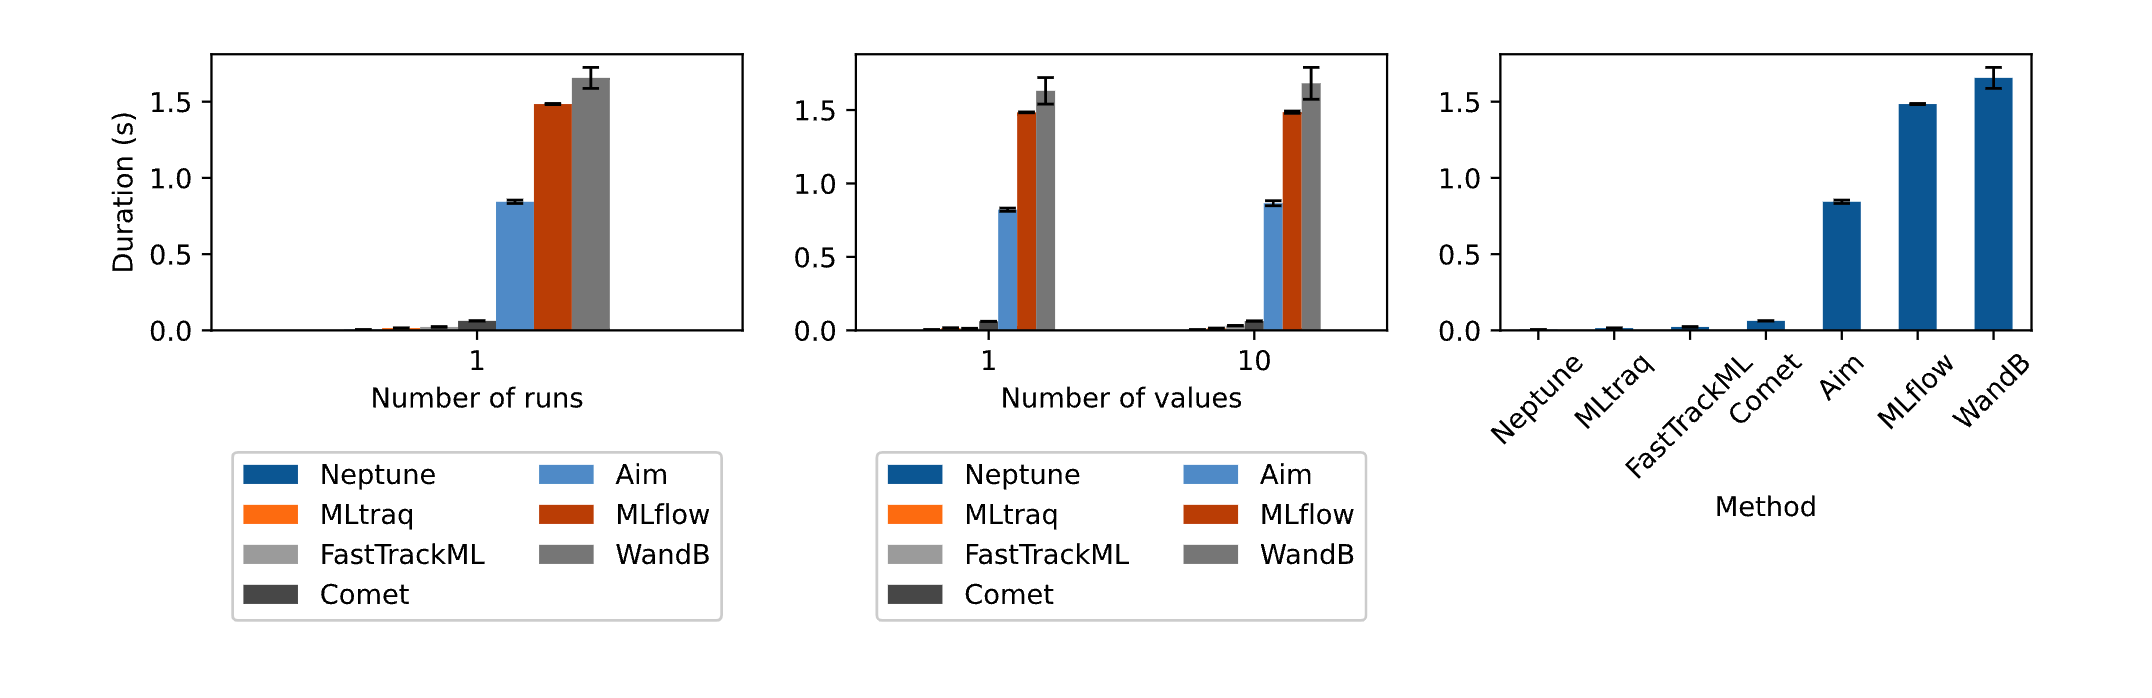
\includegraphics[width=\textwidth]{images/mltraq/mltraq-Initialization-time.png}
    \caption{Initialization time for tracking a single value across different experiment tracking solutions.}
    \label{fig:init-time}
\end{figure}

The results, shown in Figure \ref{fig:init-time}, indicate the following:

\begin{itemize}
    \item \textbf{WandB and MLflow:} These tools perform the worst due to threading and event management, costing up to 400 times more than the other methods.
    \item \textbf{Aim:} Spends most of the time creating and managing its embedded key-value store.
    \item \textbf{Comet:} The cost is primarily due to thread management.
    \item \textbf{FastTrackML:} Remarkably fast in creating new runs due to its background server, which eliminates most of the database initialization cost.
    \item \textbf{MLtraq:} Writing to SQLite is the primary cost.
    \item \textbf{Neptune:} Performs best with no threading, no SQLite database, and simply writing the tracking data to files.\newline
\end{itemize}

\textbf{Experiment 2: High-Frequency Tracking}

While efficient initialization is essential, the ability to monitor many values quickly is critical for any tracking solution. This experiment assesses the time required to track and store up to 10,000 values.

\begin{figure}[h!]
    \centering
    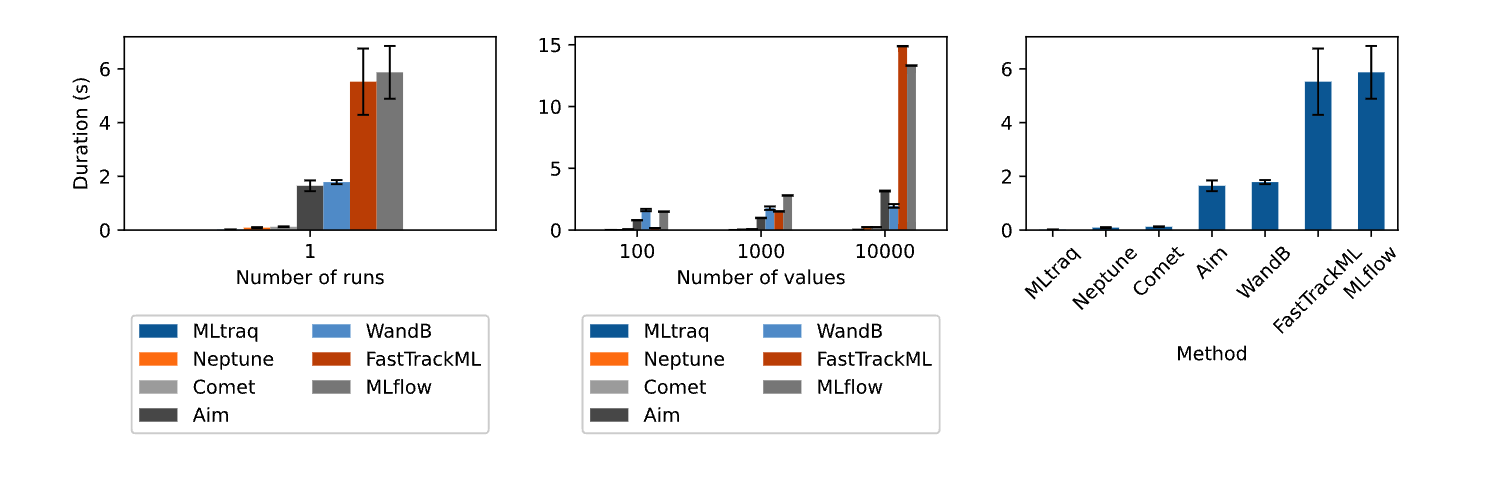
\includegraphics[width=\textwidth]{images/mltraq/mltraq-high-frequency.png}
    \caption{High-frequency tracking performance for up to 10,000 values across different experiment tracking solutions.}
    \label{fig:high-freq}
\end{figure}

The results, illustrated in Figure \ref{fig:high-freq}, highlight the following:

\begin{itemize}
    \item \textbf{FastTrackML:} While efficient in creating new runs, inserting new tracking records is similarly expensive to MLflow due to their entity-attribute-value database model.
    \item \textbf{Aim and WandB:} Perform at a fraction of the cost compared to MLflow and FastTrackML.
    \item \textbf{Neptune, Comet, and MLtraq:} These are the highest-performing methods, with MLtraq being the fastest, up to 100 times faster than WandB.\newline
\end{itemize}

\textbf{MLtraq: The Fastest Experiment-Tracking Solution}

MLtraq stands out as the fastest experiment-tracking solution for workloads involving hundreds of thousands of runs and arbitrarily large, complex Python objects. It provides superior performance and flexibility, making it an optimal choice for efficient and scalable experiment tracking.

\begin{itemize}
    \item The primary goal of other solutions often gravitates toward backward compatibility, third-party integrations, and complete model lifecycle management. However, their support for rich modeling of experiments, runs, and complex Python objects is limited or missing.
    \item Relying solely on the filesystem as a database is a recipe for low performance. As noted on the SQLite website, using a single file to store the local database copy can be 35\% faster than a filesystem-based solution. MLtraq provides the flexibility to choose where to store objects with the Data store interface.
    \item Solutions that adopt threading to incorporate streaming capabilities incur the hidden cost of Inter-Process Communication (IPC), resulting in more I/O errors and reliability concerns.
    \item The entity-attribute-value database model adopted by MLflow and FastTrackML requires inserting a new record for every new tracked value, making it painfully slow.
    \item Most methods implement the serialization of arrays and other complex, non-scalar objects with custom text encodings, relying on uuencoding and JSON-like formats. Arrow IPC, native serialization, zero-copy writes, and safe pickling provide superior performance and portability, as demonstrated by MLtraq.
\end{itemize}

Due to these significant advantages, we will analyze this innovative approach in detail.


\subsubsection{Key Features}

MLtraq includes a range of features designed to enhance the experiment tracking process:

\begin{itemize}
    \item \textbf{Immediate:} Allows the design and execution of experiments with just a few lines of code and supports metric streaming.
    \item \textbf{Collaborative:} Supports backing up, merging, sharing, and reloading experiments with their computation state anywhere.
    \item \textbf{Interoperable:} Provides access to experiments through Python, Pandas, and SQL with native database types and open formats.
    \item \textbf{Flexible:} Tracks native Python data types and structures, as well as NumPy, Pandas, and PyArrow objects.
    \item \textbf{Lightweight:} A thin layer with minimal dependencies that can run anywhere and complement other components and services.
\end{itemize}

\subsubsection{Design Choices}

MLtraq incorporates several thoughtful design choices to optimize its functionality:

\begin{itemize}
    \item \textbf{Computation:} Uses joblib.Parallel for process-based parallelism in chained execution of steps. It also supports cluster-specific backends like Dask, Ray, and Spark, requiring step functions and run objects to be serializable with cloudpickle.
    \item \textbf{Persistence:} Defaults to SQLite but can connect to any SQL database supported by SQLAlchemy. It supports a wide range of data types and provides a Data store interface for handling large objects. Compression is available but disabled by default.
\end{itemize}
\newpage


\subsection{(Maybe improved) Introduction to MLtraq: An Open-source Python Library}


MLtraq offers several key advantages:

\begin{itemize}
    \item \textbf{Blazing Fast:} Recognized as the fastest experiment tracking solution in the industry, MLtraq ensures minimal initialization times and supports high-frequency logging, which is crucial for a smooth developer experience and effective CI/CD processes. Its ability to efficiently track large, complex Python objects like datasets, time series, and media files without limitations makes it a robust and powerful tool for ML and AI development. Unlike other solutions that rely solely on the filesystem, MLtraq uses a proper database setup, which significantly improves scalability and reliability. The Data store interface provides flexibility in object storage locations.
    \item \textbf{Extreme Tracking and Interoperability:} MLtraq excels in tracking and interoperability with its unique DATAPAK format, ensuring efficient serialization and deserialization of diverse data types. DATAPAK leverages open formats like Arrow IPC for Pandas and Arrow tables, and NumPy NEP for NumPy arrays, to encode complex Python objects into manageable formats. This format, combined with the use of a safe subset of Pickle opcodes, allows seamless integration with native database types and ensures robust handling of complex objects, enhancing collaboration and data sharing capabilities across local or remote SQL databases. In contrast, the entity-attribute-value database model used by MLflow and FastTrackML requires inserting a new record for each tracked value, which is slow and inflexible.
    \item \textbf{Promoting Collaboration:} MLtraq facilitates seamless collaboration by allowing teams to create, store, reload, mix, resume, and share experiments using any local or remote SQL database. The state of experiments is persisted to the database in tables, enabling robust data management. Supported data types include native database types, basic types, container types, and complex types, all serialized with the DATAPAK format for consistency. This ensures that experiments can be easily backed up, merged, and shared, enhancing collaborative efforts across different environments and promoting efficient teamwork.
    \item \textbf{Flexible and Open:} MLtraq enables interaction with experiments using Python, Pandas, and SQL, providing flexibility without vendor lock-in. Most methods implement the serialization of arrays and other complex, non-scalar objects with custom text encodings, relying on uuencoding and JSON-like formats. Compression is either missing or handled by creating ZIP files of artifacts stored on the filesystem. The process is slow, and the support for complex types is limited or missing: floating point and timestamp precision are ignored, etc. Arrow IPC, native serialization, zero-copy writes, and safe pickling provide superior performance and portability, as demonstrated by MLtraq.
\end{itemize}

\subsubsection{Performance Evaluation of Experiment Tracking Solutions}

We conducted two experiments to evaluate the performance of various experiment tracking solutions, including MLtraq, Weights \& Biases (W\&B), Neptune, FastTrackML, Comet, Aim, and MLflow. The experiments focused on initialization time and high-frequency tracking performance.

\textbf{Experiment 1: Initialization Time}

This experiment measures the time required to start a new experiment and track a single value. Initialization time is a critical factor, as it impacts the ability to experiment with hundreds of thousands of possible configurations. The primary costs are dominated by threading and database management.

\begin{figure}[h!]
    \centering
    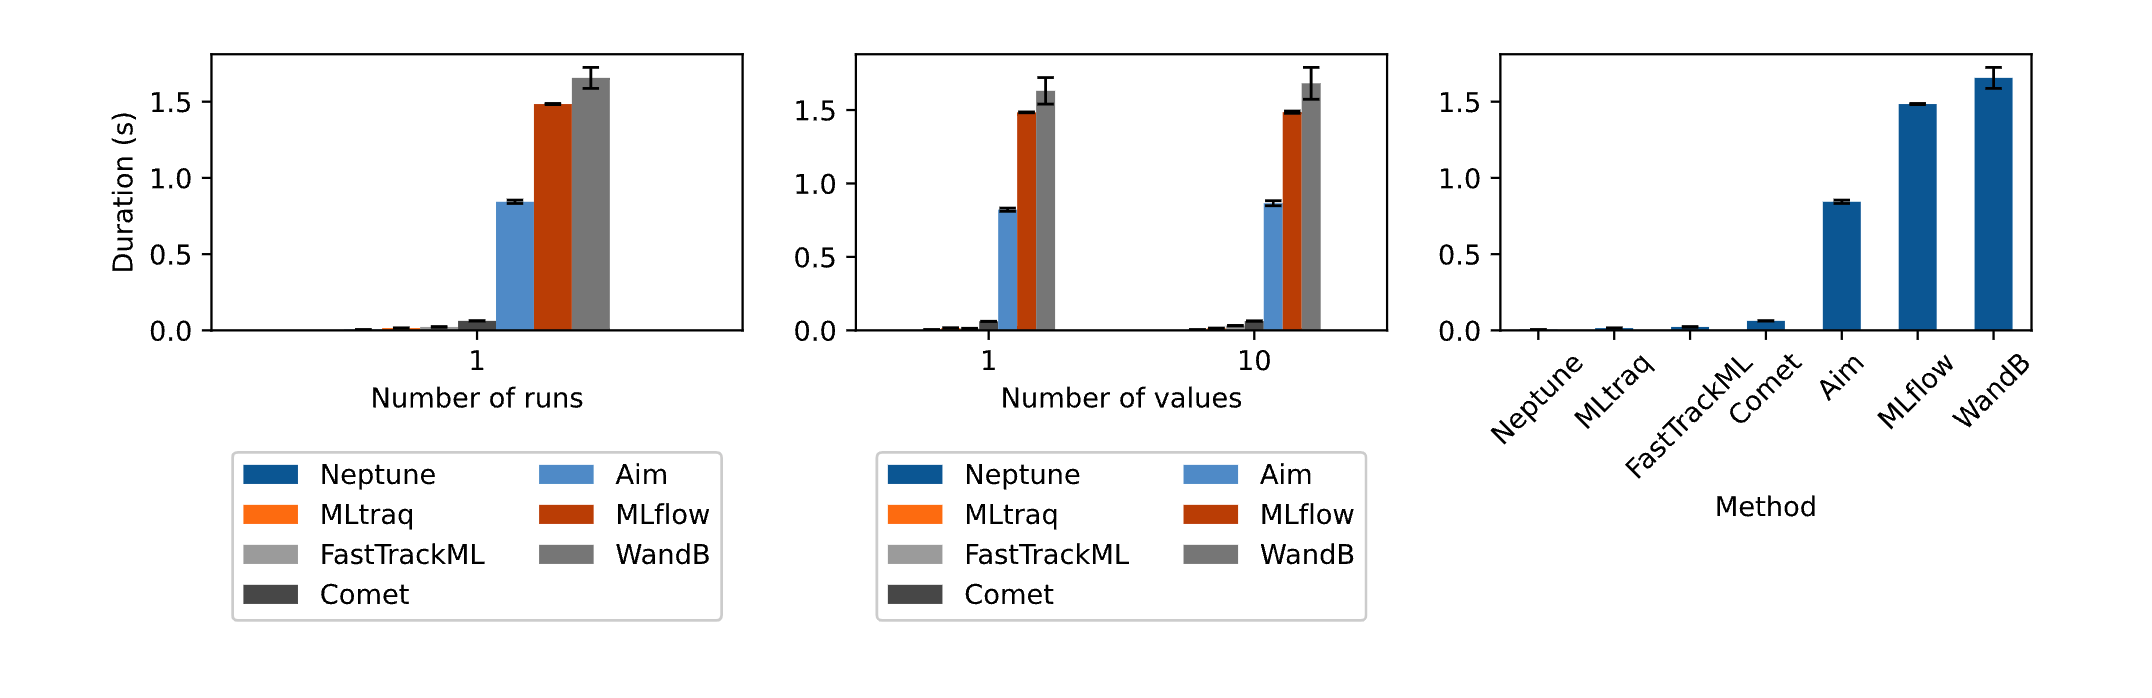
\includegraphics[width=\textwidth]{images/mltraq/mltraq-Initialization-time.png}
    \caption{Initialization time for tracking a single value across different experiment tracking solutions.}
    \label{fig:init-time}
\end{figure}

The results, shown in Figure \ref{fig:init-time}, indicate the following:

\begin{itemize}
    \item \textbf{WandB and MLflow:} These tools perform the worst due to threading and event management, costing up to 400 times more than the other methods.
    \item \textbf{Aim:} Spends most of the time creating and managing its embedded key-value store.
    \item \textbf{Comet:} The cost is primarily due to thread management.
    \item \textbf{FastTrackML:} Remarkably fast in creating new runs due to its background server, which eliminates most of the database initialization cost.
    \item \textbf{MLtraq:} Writing to SQLite is the primary cost.
    \item \textbf{Neptune:} Performs best with no threading, no SQLite database, and simply writing the tracking data to files.
\end{itemize}

\textbf{Experiment 2: High-Frequency Tracking}

While efficient initialization is essential, the ability to monitor many values quickly is critical for any tracking solution. This experiment assesses the time required to track and store up to 10,000 values.

\begin{figure}[h!]
    \centering
    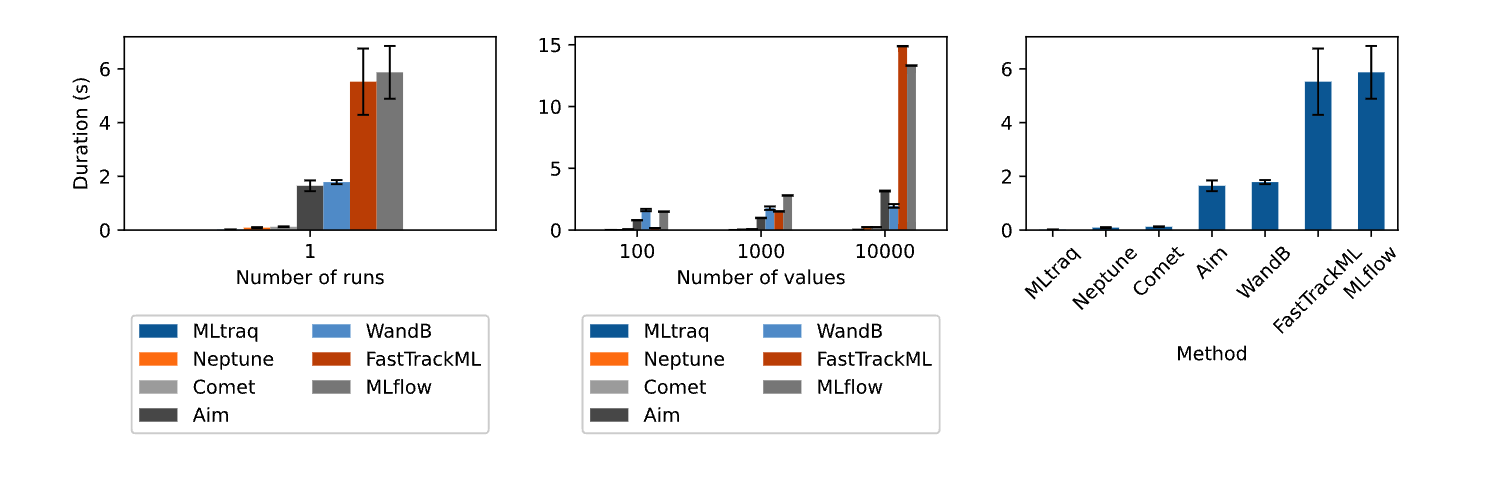
\includegraphics[width=\textwidth]{images/mltraq/mltraq-high-frequency.png}
    \caption{High-frequency tracking performance for up to 10,000 values across different experiment tracking solutions.}
    \label{fig:high-freq}
\end{figure}

The results, illustrated in Figure \ref{fig:high-freq}, highlight the following:

\begin{itemize}
    \item \textbf{FastTrackML:} While efficient in creating new runs, inserting new tracking records is similarly expensive to MLflow due to their entity-attribute-value database model.
    \item \textbf{Aim and WandB:} Perform at a fraction of the cost compared to MLflow and FastTrackML.
    \item \textbf{Neptune, Comet, and MLtraq:} These are the highest-performing methods, with MLtraq being the fastest, up to 100 times faster than WandB.
\end{itemize}

\textbf{MLtraq: The Fastest Experiment-Tracking Solution}

MLtraq stands out as the fastest experiment-tracking solution for workloads involving hundreds of thousands of runs and arbitrarily large, complex Python objects. It provides superior performance and flexibility, making it an optimal choice for efficient and scalable experiment tracking.

\begin{itemize}
    \item The primary goal of other solutions often gravitates toward backward compatibility, third-party integrations, and complete model lifecycle management. However, their support for rich modeling of experiments, runs, and complex Python objects is limited or missing.
    \item Relying solely on the filesystem as a database is a recipe for low performance. As noted on the SQLite website, using a single file to store the local database copy can be 35\% faster than a filesystem-based solution. MLtraq provides the flexibility to choose where to store objects with the Data store interface.
    \item Solutions that adopt threading to incorporate streaming capabilities incur the hidden cost of Inter-Process Communication (IPC), resulting in more I/O errors and reliability concerns.
    \item The entity-attribute-value database model adopted by MLflow and FastTrackML requires inserting a new record for every new tracked value, making it painfully slow.
    \item Most methods implement the serialization of arrays and other complex, non-scalar objects with custom text encodings, relying on uuencoding and JSON-like formats. Arrow IPC, native serialization, zero-copy writes, and safe pickling provide superior performance and portability, as demonstrated by MLtraq.
\end{itemize}

Due to these significant advantages, we will analyze this innovative approach in detail.

\subsubsection{Key Features}

MLtraq includes a range of features designed to enhance the experiment tracking process:

\begin{itemize}
    \item \textbf{Immediate:} Allows the design and execution of experiments with just a few lines of code and supports metric streaming.
    \item \textbf{Collaborative:} Supports backing up, merging, sharing, and reloading experiments with their computation state anywhere.
    \item \textbf{Interoperable:} Provides access to experiments through Python, Pandas, and SQL with native database types and open formats.
    \item \textbf{Flexible:} Tracks native Python data types and structures, as well as NumPy, Pandas, and PyArrow objects.
    \item \textbf{Lightweight:} A thin layer with minimal dependencies that can run anywhere and complement other components and services.
\end{itemize}

\subsubsection{Design Choices}

MLtraq incorporates several thoughtful design choices to optimize its functionality:

\begin{itemize}
    \item \textbf{Computation:} Uses joblib.Parallel for process-based parallelism in chained execution of steps. It also supports cluster-specific backends like Dask, Ray, and Spark, requiring step functions and run objects to be serializable with cloudpickle.
    \item \textbf{Persistence:} Defaults to SQLite but can connect to any SQL database supported by SQLAlchemy. It supports a wide range of data types and provides a Data store interface for handling large objects. Compression is available but disabled by default.
\end{itemize}


\newpage

\section{State-of-the-art Models}
Selection of state-of-the-art LLMs (GPT-4o, Claude 3.5, Gemini Pro, Mistral, Meta Llama 3,...) to compare their differences in performance, architecture, accessibility and cost for developing question-answering chatbot systems.

\subsection{Challenges and Limitations}
Discussion on cost, carbon footprint and energy consumption and privacy concerns.

\subsection{Beyond Transformers: the Mamba LLM Architecture}
Discover the power of Mamba LLM, a transformative architecture from leading universities, redefining sequence processing in AI.

